%\documentclass{standalone}

%\usepackage[T1]{fontenc}
\usepackage{amsmath,amssymb,mathtools}
\newcommand{\set}[1]{\left\{ #1 \right \}}

%\usepackage{graphicx}
%\definecolor{navyblue}{RGB}{0,0,128}

%\begin{document}

	\begin{tikzpicture}[node distance=1.45cm,  minimum
	  height=0.7cm,font=\scriptsize] 

        \node[] (l0) {{\scriptsize {\bf Input}}};
	\node[right of =l0, xshift=11.25em] (1) {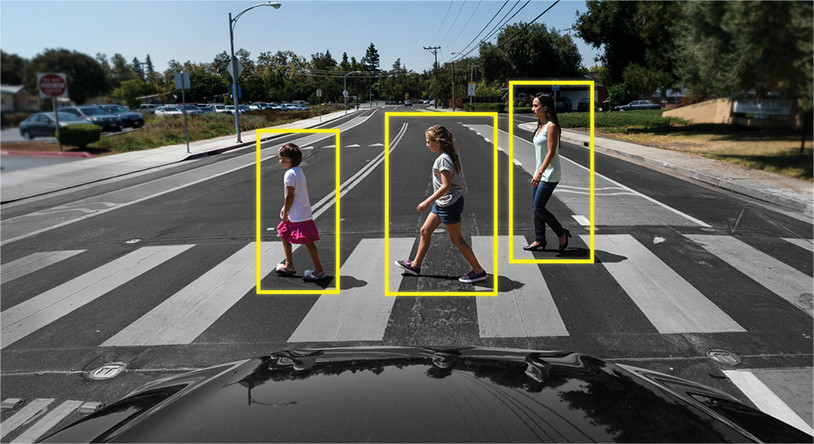
\includegraphics[width=1.4cm]{images/pedestrian.jpg}};
    \node[below of=1, yshift=2.25em] (x1) {{\large $\downarrow$}};

        \node[below of = l0] (l1) {{\scriptsize{\bf Perturbations}}};
        \node[label={[below, yshift=-2em]{\scriptsize Brightness}}, right of=l1,below of =l0, xshift=1em] (2) {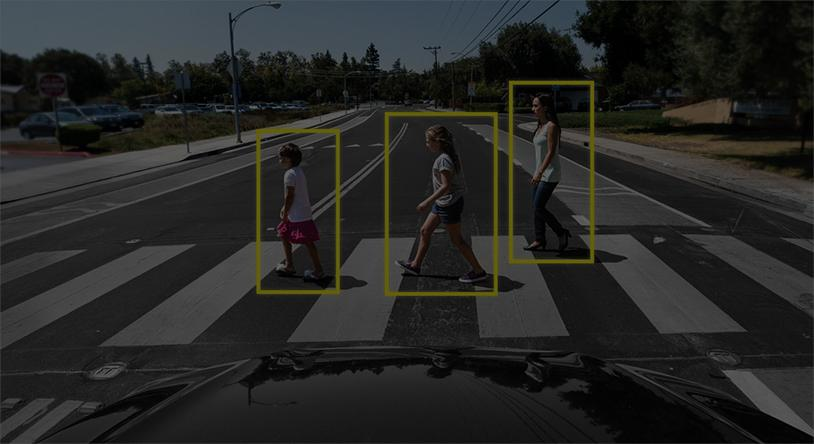
\includegraphics[width=1.4cm]{images/pedestrian_brightness.jpg}};
        \node[label={[below, yshift=-2em]{\scriptsize Contrast}}, right of =2] (3) {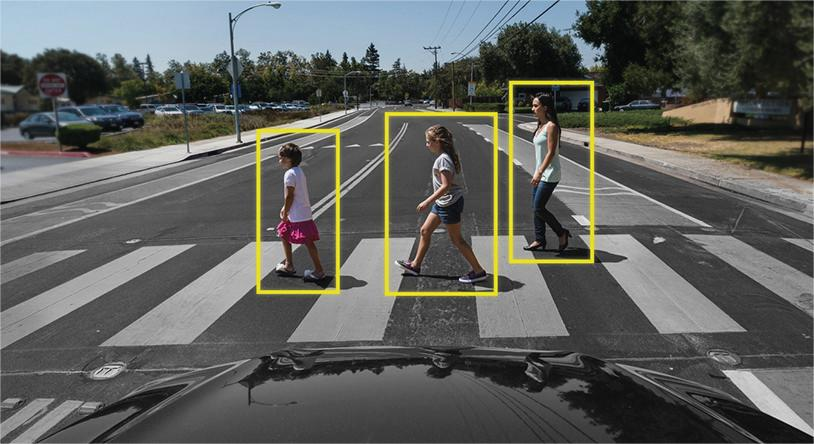
\includegraphics[width=1.4cm]{images/pedestrian_contrast.jpg}};
        \node[label={[below, yshift=-2em] {\scriptsize White noise}}, right of =3] (4) {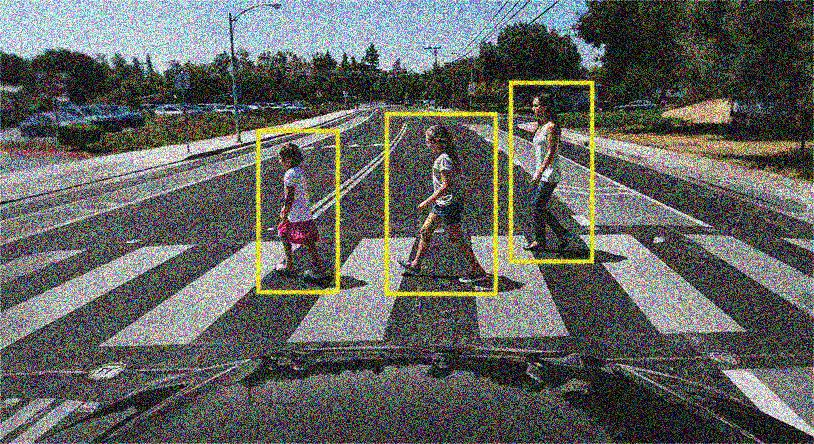
\includegraphics[width=1.4cm]{images/pedestrian_noise.jpg}};  
        \node[label={[below, yshift=-2em] {\scriptsize Rotate}}, right of =4] (5) {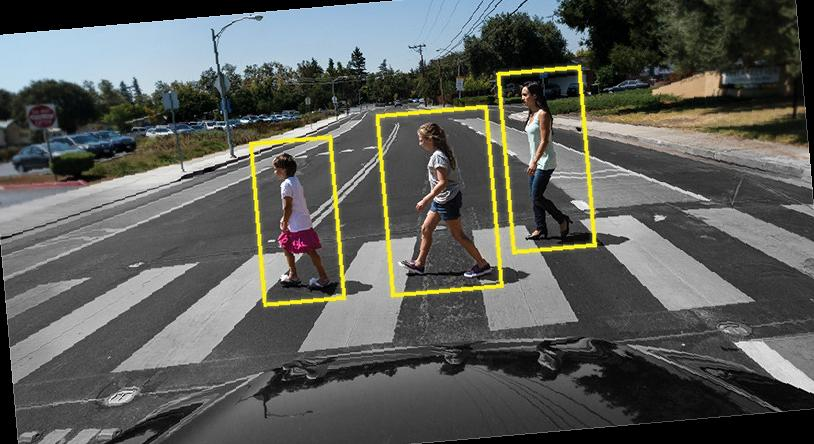
\includegraphics[width=1.4cm]{images/pedestrian_rotate.jpg}};
        \node[label={[below, yshift=-2em] {\scriptsize Scale}}, right of =5] (6) {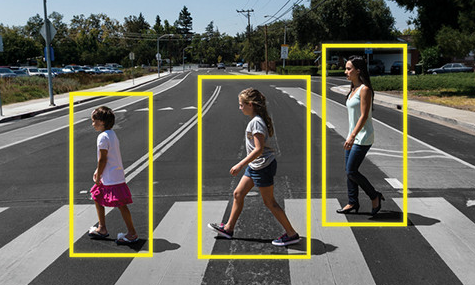
\includegraphics[width=1.3cm]{images/pedestrian_scale.png}};
        \node[label={[below, yshift=-2em] {\scriptsize Hue}}, right of =6] (7) {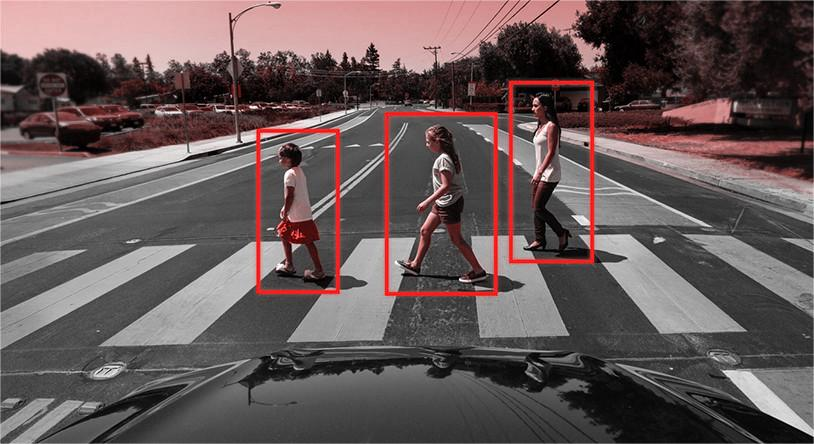
\includegraphics[width=1.4cm]{images/pedestrian_hue.jpg}};



        \node[below of = l1] (l2) {{\scriptsize{\bf Verification}}};

        \node[below of = x1, yshift=-1em] (x2) {{\large $\downarrow$}};
        \node[fig, fill=white, minimum width=3cm,rectangle, rounded corners, below of=x2, yshift=2.3em] (v) {{\bf Verification tool}};
        \node[left  of = v, xshift=-1.25em] (x4) {{\large $\rightarrow$}};
        \node[left of = x4, xshift=1.25em] (x3) {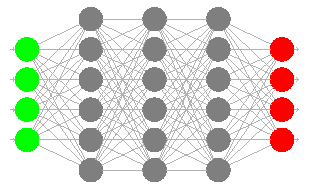
\includegraphics[width=0.15\textwidth]{images/neuralagent.pdf}};

        \node[below of = v, yshift=2em] (x2) {{\large $\downarrow$}};
        \node[below of = l2, yshift=-2em, align=center] (l3) {{\scriptsize{\bf Certification /}} \\ {\scriptsize {\bf Fragilities}}};

        \node[rectangle, fill=green!30, below of =2, yshift=-5em] {Robust};
        \node[rectangle, fill=red!30, below of =3, yshift=-5em] (y1) {Not robust};
        \node[below of = y1, yshift=1.9em] (x3) {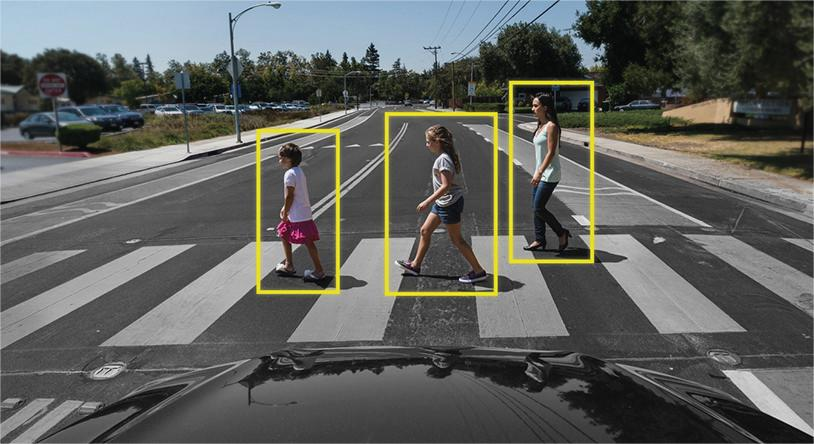
\includegraphics[width=0.13\textwidth]{images/pedestrian_contrast.jpg}};
        \node[rectangle, fill=green!30, below of =4, yshift=-5em] {Robust};
        \node[rectangle, fill=green!30, below of =5, yshift=-5em] {Robust};
        \node[rectangle, fill=red!30, below of =6, yshift=-5em] (y2) {Not robust};
        \node[below of = y2, yshift=1.9em] (x3) {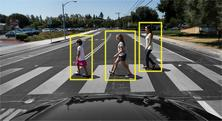
\includegraphics[width=0.13\textwidth]{images/pedestrian_scale.jpg}};
        \node[rectangle, fill=green!30, below of =7, yshift=-5em]{Robust};

        
  \path[-latex,semithick,every node/.style={->,font=\sffamily\normalsize, scale=0.9}]
        (l0) edge (l1)
        (l1) edge (l2)
        (l2) edge (l3);
        
        \node[fit=(1)(2)(7)(x3), draw=navyblue, line width=0.025cm, inner sep=0em] {};

  \end{tikzpicture}
%\end{document}
